\subsection{Dual Simulation: Cobweb and Fishery}
\label{section:fc_dual_sim}

The chapter compares seven learning paradigms on two single-agent economic decision problems. The first is a cobweb model with adjustment cost, a self-referential environment in which the agent's own action moves the contemporaneous price. The second is a logistic-growth fishery, an exogenous environment in which the agent's action depletes a renewable stock but does not feed back through expectations. The seven paradigms are an oracle that knows the true parameters, a constant-rule baseline that does not learn, recursive least squares adaptive learning \citep{MarcetSargent1989}, the genetic algorithm of \citet{Arifovic1994} without the election operator, tabular Q-learning \citep{WatkinsDayan1992}, a model-based learner that estimates demand and cost coefficients by least squares and plans through the closed-form linear-quadratic Bellman equation, and the full MBPO of \citet{janner2019model} with bootstrap-ensemble dynamics, branched rollouts, and a linear policy trained by REINFORCE. The experiment is deliberately favorable to structured learners; the two environments have low-dimensional state, smooth payoffs, and stable parametric form, and the purpose is to locate the methods on an inductive-bias frontier rather than to rank them universally.

\subsubsection{Cobweb with adjustment cost}
\label{section:fc_dual_sim_cobweb}

The cobweb panel is designed to expose three things in turn: where each paradigm sits on the inductive-bias-vs-data trade-off, how parameter recovery rates differ across regimes, and where regret performance and policy quality come apart for methods that bake in correct functional form. The cobweb stability parameter $b/c$ varies across regimes to modulate the curvature of the value function rather than to drive the kind of E-stability divergence \citet{MarcetSargent1989} report for the multi-agent expectational cobweb, which does not arise in this single-agent monopoly variant.

\paragraph*{Setup.}%
The state is $s_t = (q_{t-1}, p_{t-1}) \in \mathbb{R}^2$ and the action is $q_t \in [0, 4]$. The price clears contemporaneously as $p_t = a - b q_t + \varepsilon_t$ with $\varepsilon_t \sim \mathcal{N}(0, \sigma^2)$, and the reward is $r_t = p_t q_t - (c/2) q_t^2 - (\phi/2)(q_t - q_{t-1})^2$, so the agent faces a linear demand, a quadratic production cost, and a quadratic adjustment cost. The sweep is $b/c \in \{0.5, 1.0, 2.0\}$ with $a = 4$, $c = 1$, $\phi = 0.2$, $\sigma = 0.1$, $\gamma = 0.95$, $T = 500$, and twenty independent seeds. The oracle policy is the affine feedback rule $q_t^\star = K_0 + K_q q_{t-1}$ recovered by quadratic-form fixed-point iteration on the Bellman equation, and cumulative regret is computed per seed against the oracle's realized return on the same noise sequence.

\paragraph*{Models.}%
Seven paradigms share the budget. The oracle knows $(a, b, c, \phi)$ and applies the closed-form optimal feedback rule. The constant-rule baseline plays $q_t = 1.4$ at every step regardless of state, providing the absolute no-learning floor. Recursive least squares of \citet{MarcetSargent1989} estimates $(\hat a, \hat b)$ from observed prices, treats $(c, \phi)$ as known, and re-solves the linear-quadratic planner with point estimates each period. The genetic algorithm of \citet{Arifovic1994} maintains a population of binary-encoded production rules, evolves them under fitness-proportional selection on the running mean of realized observed profit, single-point crossover, bit-flip mutation, and two-elite preservation, and plays the population's incumbent rule; the original Arifovic 1994 election operator scored hypothetical offspring against their parents using the true demand and cost parameters, and is omitted here so the agent uses only realized observed profit. Tabular Q-learning of \citet{WatkinsDayan1992} discretizes the state-action space onto a $20 \times 20 \times 25$ grid and applies $\varepsilon$-greedy temporal-difference updates with $\alpha = 0.1$ and $\varepsilon$ decaying linearly from $0.3$ to $0.01$. Two model-based learners share the same parameter-estimation step but differ in how they plan. The model-based LQ learner exploits the linear-Gaussian structure: it solves the closed-form linear-quadratic Bellman equation by Riccati iteration on current point estimates of $(\hat a, \hat b, \hat c, \hat \phi)$ each step and acts under the resulting affine feedback rule with Gaussian exploration noise. The MBPO learner of \citet{janner2019model} maintains a bootstrap ensemble of five linear-Gaussian demand models, parameterizes the policy as $q = K_0 + K_q q_{t-1}$, and at each real step samples ten rollouts of horizon five from buffer-uniform initial states under random ensemble members, accumulating discounted returns from the learned reward model and updating $(K_0, K_q)$ by REINFORCE with a moving-average baseline.

\paragraph*{Results.}%
Table~\ref{table:fc_cobweb_results} reports cumulative regret at $T = 500$ for each paradigm and regime; Figure~\ref{figure:fc_cobweb_curves} shows the corresponding regret trajectories. Paradigms are presented in rank order by mean regret across regimes. Recursive least squares attains regret of about five units, indistinguishable across regimes within standard error, because it has the correct functional form for the price map and known cost parameters and need only estimate the two demand coefficients. The model-based LQ learner trails by an order of magnitude with regret rising from about twelve to forty-three units as the regime moves from stable to unstable, reflecting the larger curvature it must resolve in the unstable region and the additional cost coefficients it must learn alongside the demand map. The genetic algorithm of \citet{Arifovic1994} without the election operator is a further order of magnitude behind, with regret of ninety to three hundred units, reflecting the cost of gradient-free population search over a binary chromosome with no parametric knowledge of demand or cost. The constant rule shifts with the regime in a way that reflects the position of the fixed action relative to the regime's optimum and is included as the absolute no-learning floor, not as a learning competitor. The full MBPO learner of \citet{janner2019model} sits next, with regret that varies more than two orders of magnitude across regimes (six hundred and fifty in stable, one hundred and twelve in borderline, forty-nine in unstable); the variance reflects REINFORCE's sensitivity to the curvature of the return surface, which is flat in the stable regime where small differences in $(K_0, K_q)$ matter little for return and sharp in the unstable regime where the policy gradient carries usable signal. Tabular Q-learning finishes near a thousand units of regret in every regime, the empirical signature of model-free tabular methods in continuous problems under a tight environment budget. The take-away is that on this cobweb, under the present hyperparameters, branched-rollout REINFORCE underperforms closed-form planning across all three regimes, with the gap widest in the stable regime where the return surface is flattest for the REINFORCE gradient estimator. The two methods share the same parameter-estimation step; the difference is what the planner does with the point estimates.

Regret captures the integrated cost of learning, not the asymptotic quality of the recovered model or policy. Figure~\ref{figure:fc_cobweb_recovery} plots the parameter trajectories $\hat a_t$ and $\hat b_t$ for recursive least squares, the model-based LQ learner, and the MBPO ensemble mean against the true values, and Table~\ref{table:fc_cobweb_recovery} reports the final $|\hat\theta - \theta|$ error per paradigm and regime. All three methods recover the demand coefficients to within four percent of the truth in every regime; the two model-based learners additionally recover the cost coefficients $(c, \phi)$ to within machine precision\footnote{The exact recovery reflects noiseless reward in this simulation: given observed $(p_t, q_t, q_{t-1})$, the equation $r_t = p_t q_t - (c/2) q_t^2 - (\phi/2)(q_t - q_{t-1})^2$ is exactly solvable for $(c, \phi)$ from any two tuples that span the cost feature space. With additive reward noise $\sigma_r > 0$, recovery would degrade at rate $O(\sigma_r / \sqrt{N})$.} because the reward signal pins them down once the residual $r_t - p_t q_t$ is regressed on $(q_t^2, (q_t - q_{t-1})^2)$. Recovery is fastest in the unstable regime because the curvature of the demand map sharpens the information content of each observation; this is the same observation that explains why the regret values themselves are similar across regimes even though the absolute return at the oracle's policy is lower in the unstable regime.

Figure~\ref{figure:fc_cobweb_policy_distance} reports the distance from each learner's noise-free action at a regime-specific reference state to the oracle's action at the same state, on a log scale. The ordering is by inductive bias rather than recovery accuracy. The model-based LQ learner attains the smallest residual policy distance in every regime, two to three times smaller than recursive least squares in absolute terms, because by estimating $(c, \phi)$ it places its planner at the correct curvature of the value function. Recursive least squares is bounded below by the discrepancy between the prior on $(c, \phi)$ that fixes its planner and the realized environment, which is small here only because the prior was chosen to match. The genetic algorithm tracks a policy distance an order of magnitude larger, reflecting the discretization of the chromosome over the action space rather than incomplete recovery of any continuous parameter. The MBPO learner sits between the genetic algorithm and tabular Q-learning in the stable regime where REINFORCE has not converged its linear policy, and approaches the model-based LQ learner's accuracy in the unstable regime where the gradient signal is strong; this regime dependence is the practical cost of the REINFORCE update relative to the analytical planner. Tabular Q-learning sits at order one, a direct consequence of the coarseness of the action grid (twenty-five points over a range of four units) compounded by the constant exploration noise injected into the rollout. The constant rule is flat by construction at a value that depends on how far the fixed action $q_{\text{fixed}} = 1.4$ lies from the regime's optimum, and the value distinguishes how much of the no-learning floor is luck of the regime rather than any property of learning.

The verdict is that recursive least squares wins the regret comparison because its early decisions are nearly optimal under correct functional form and known cost parameters, while the model-based LQ learner wins the asymptotic policy-distance comparison because it ultimately fits more of the problem's structure; the two methods occupy adjacent positions on the inductive-bias frontier, with recursive least squares paying a higher per-step penalty as long as its cost-parameter prior is correct and the model-based LQ learner paying a transient information cost in exchange for a tighter asymptote. The MBPO learner with branched rollouts and REINFORCE is the third position on this frontier: same model-estimation step as the LQ learner, but a slower policy update that pays off only when the closed-form structure is unavailable. On this cobweb the closed-form structure is available and the comparison favors the LQ learner; in environments where it is not, the comparison would invert.

\begin{figure}[ht]
  \centering
  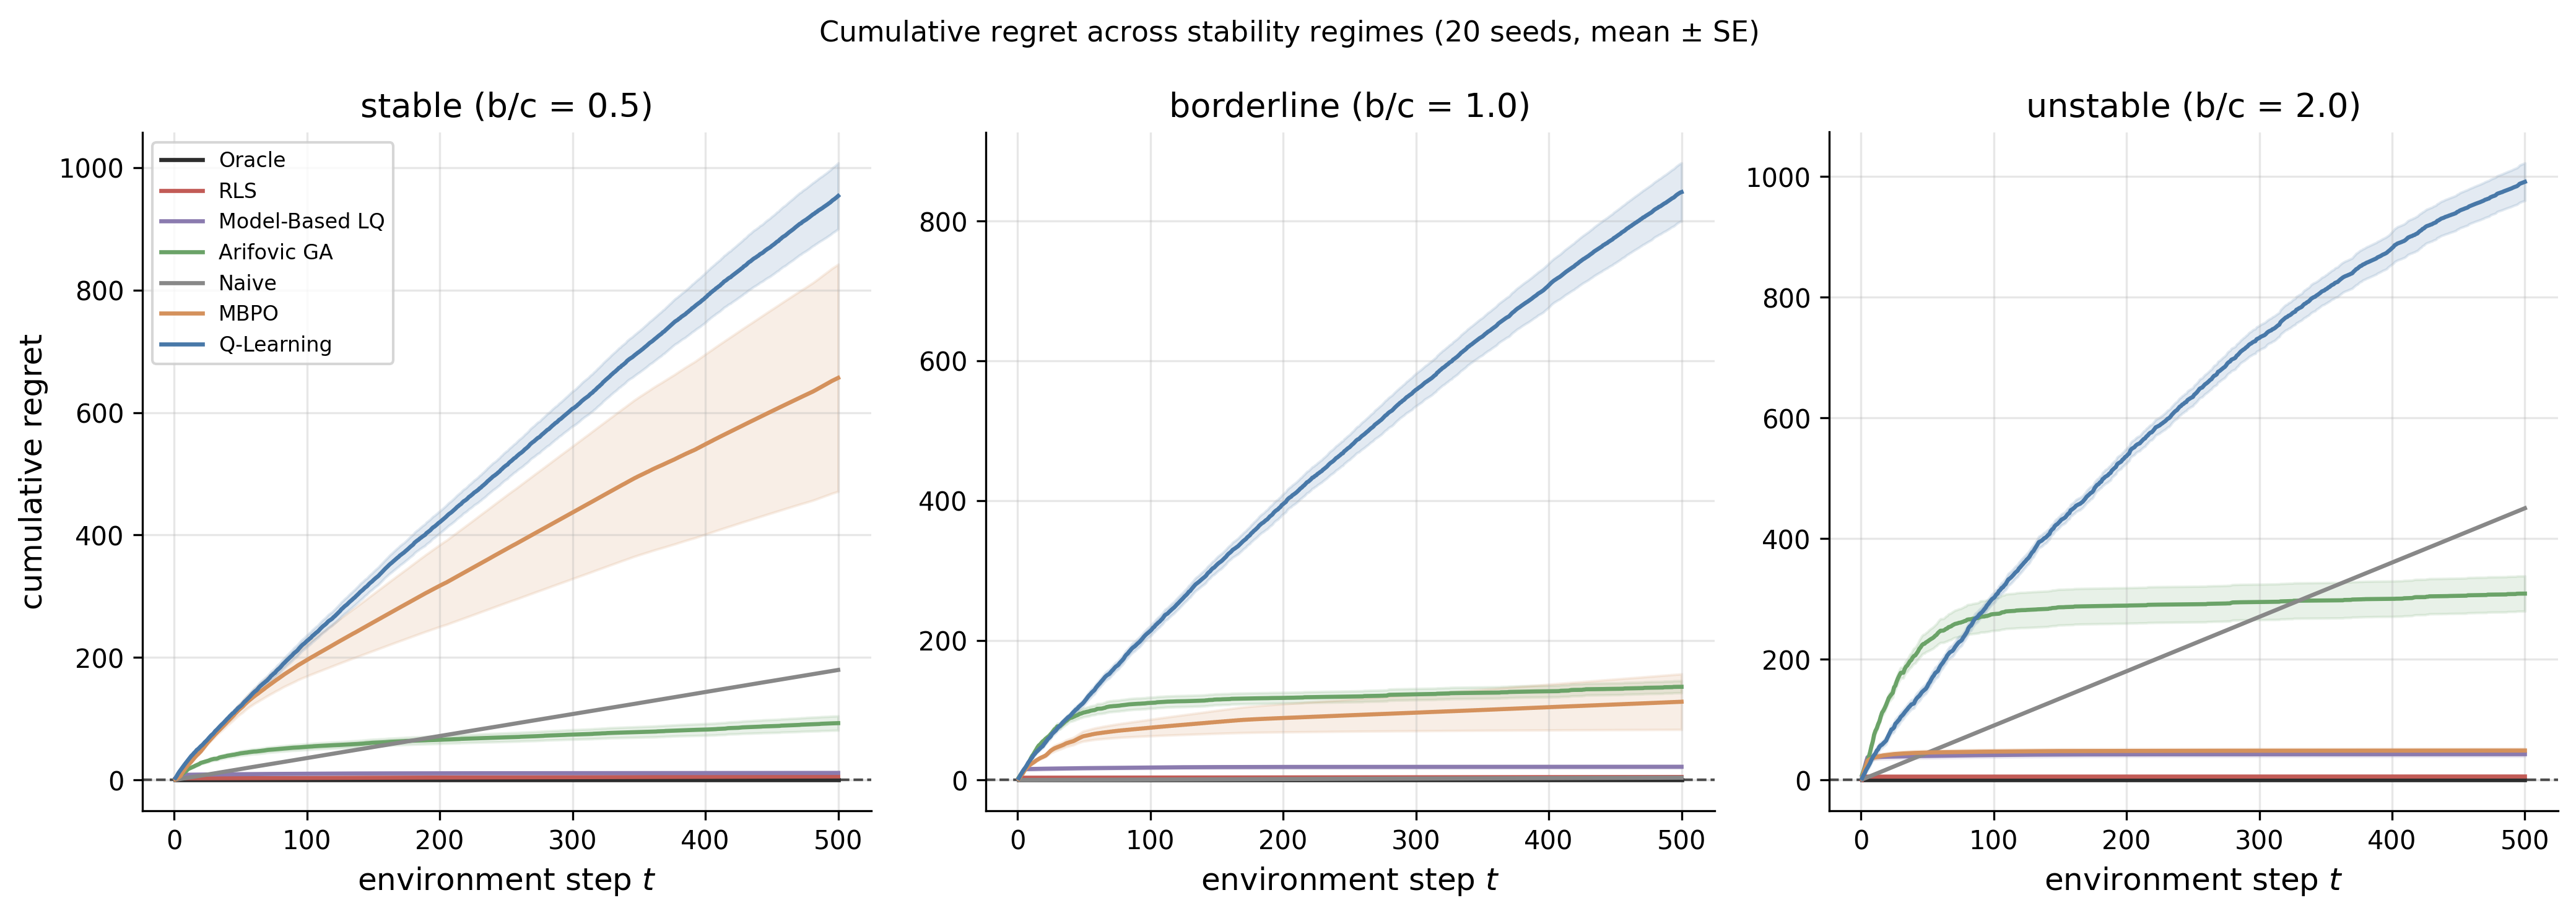
\includegraphics[width=\textwidth]{../ch12_world_models/sims/cobweb_paradigms.png}
  \caption{Cumulative regret across stability regimes for seven learning paradigms on the cobweb with adjustment cost. Lines are means and shaded bands are one standard error across twenty seeds. Panels correspond to $b/c \in \{0.5, 1.0, 2.0\}$. Oracle is the zero reference.}
  \label{figure:fc_cobweb_curves}
\end{figure}

\begin{table}[ht]
  \centering
  \caption{Cumulative regret at $T = 500$ on the cobweb with adjustment cost, mean $\pm$ standard error across twenty seeds. Lower is better; Oracle is the reference.}
  \label{table:fc_cobweb_results}
  % Cumulative regret at T=500, mean ± SE across 20 seeds.
\begin{tabular}{lrrr}
\toprule
Paradigm & Stable ($b/c=0.5$) & Borderline ($b/c=1.0$) & Unstable ($b/c=2.0$) \\
\midrule
Oracle & 0.00 $\pm$ 0.00 & 0.00 $\pm$ 0.00 & 0.00 $\pm$ 0.00 \\
RLS & 5.89 $\pm$ 1.04 & 4.38 $\pm$ 0.43 & 5.87 $\pm$ 0.18 \\
Model-Based LQ & 11.65 $\pm$ 0.93 & 18.96 $\pm$ 1.73 & 42.90 $\pm$ 3.75 \\
Arifovic GA & 92.89 $\pm$ 11.69 & 133.43 $\pm$ 8.65 & 308.88 $\pm$ 29.16 \\
Naive & 179.73 $\pm$ 0.34 & 3.37 $\pm$ 0.04 & 450.34 $\pm$ 0.34 \\
MB-LG-REINFORCE & 656.60 $\pm$ 185.41 & 112.06 $\pm$ 39.78 & 48.87 $\pm$ 3.47 \\
Q-Learning & 953.69 $\pm$ 53.79 & 841.50 $\pm$ 41.63 & 991.15 $\pm$ 31.19 \\
\bottomrule
\end{tabular}

\end{table}

\begin{figure}[ht]
  \centering
  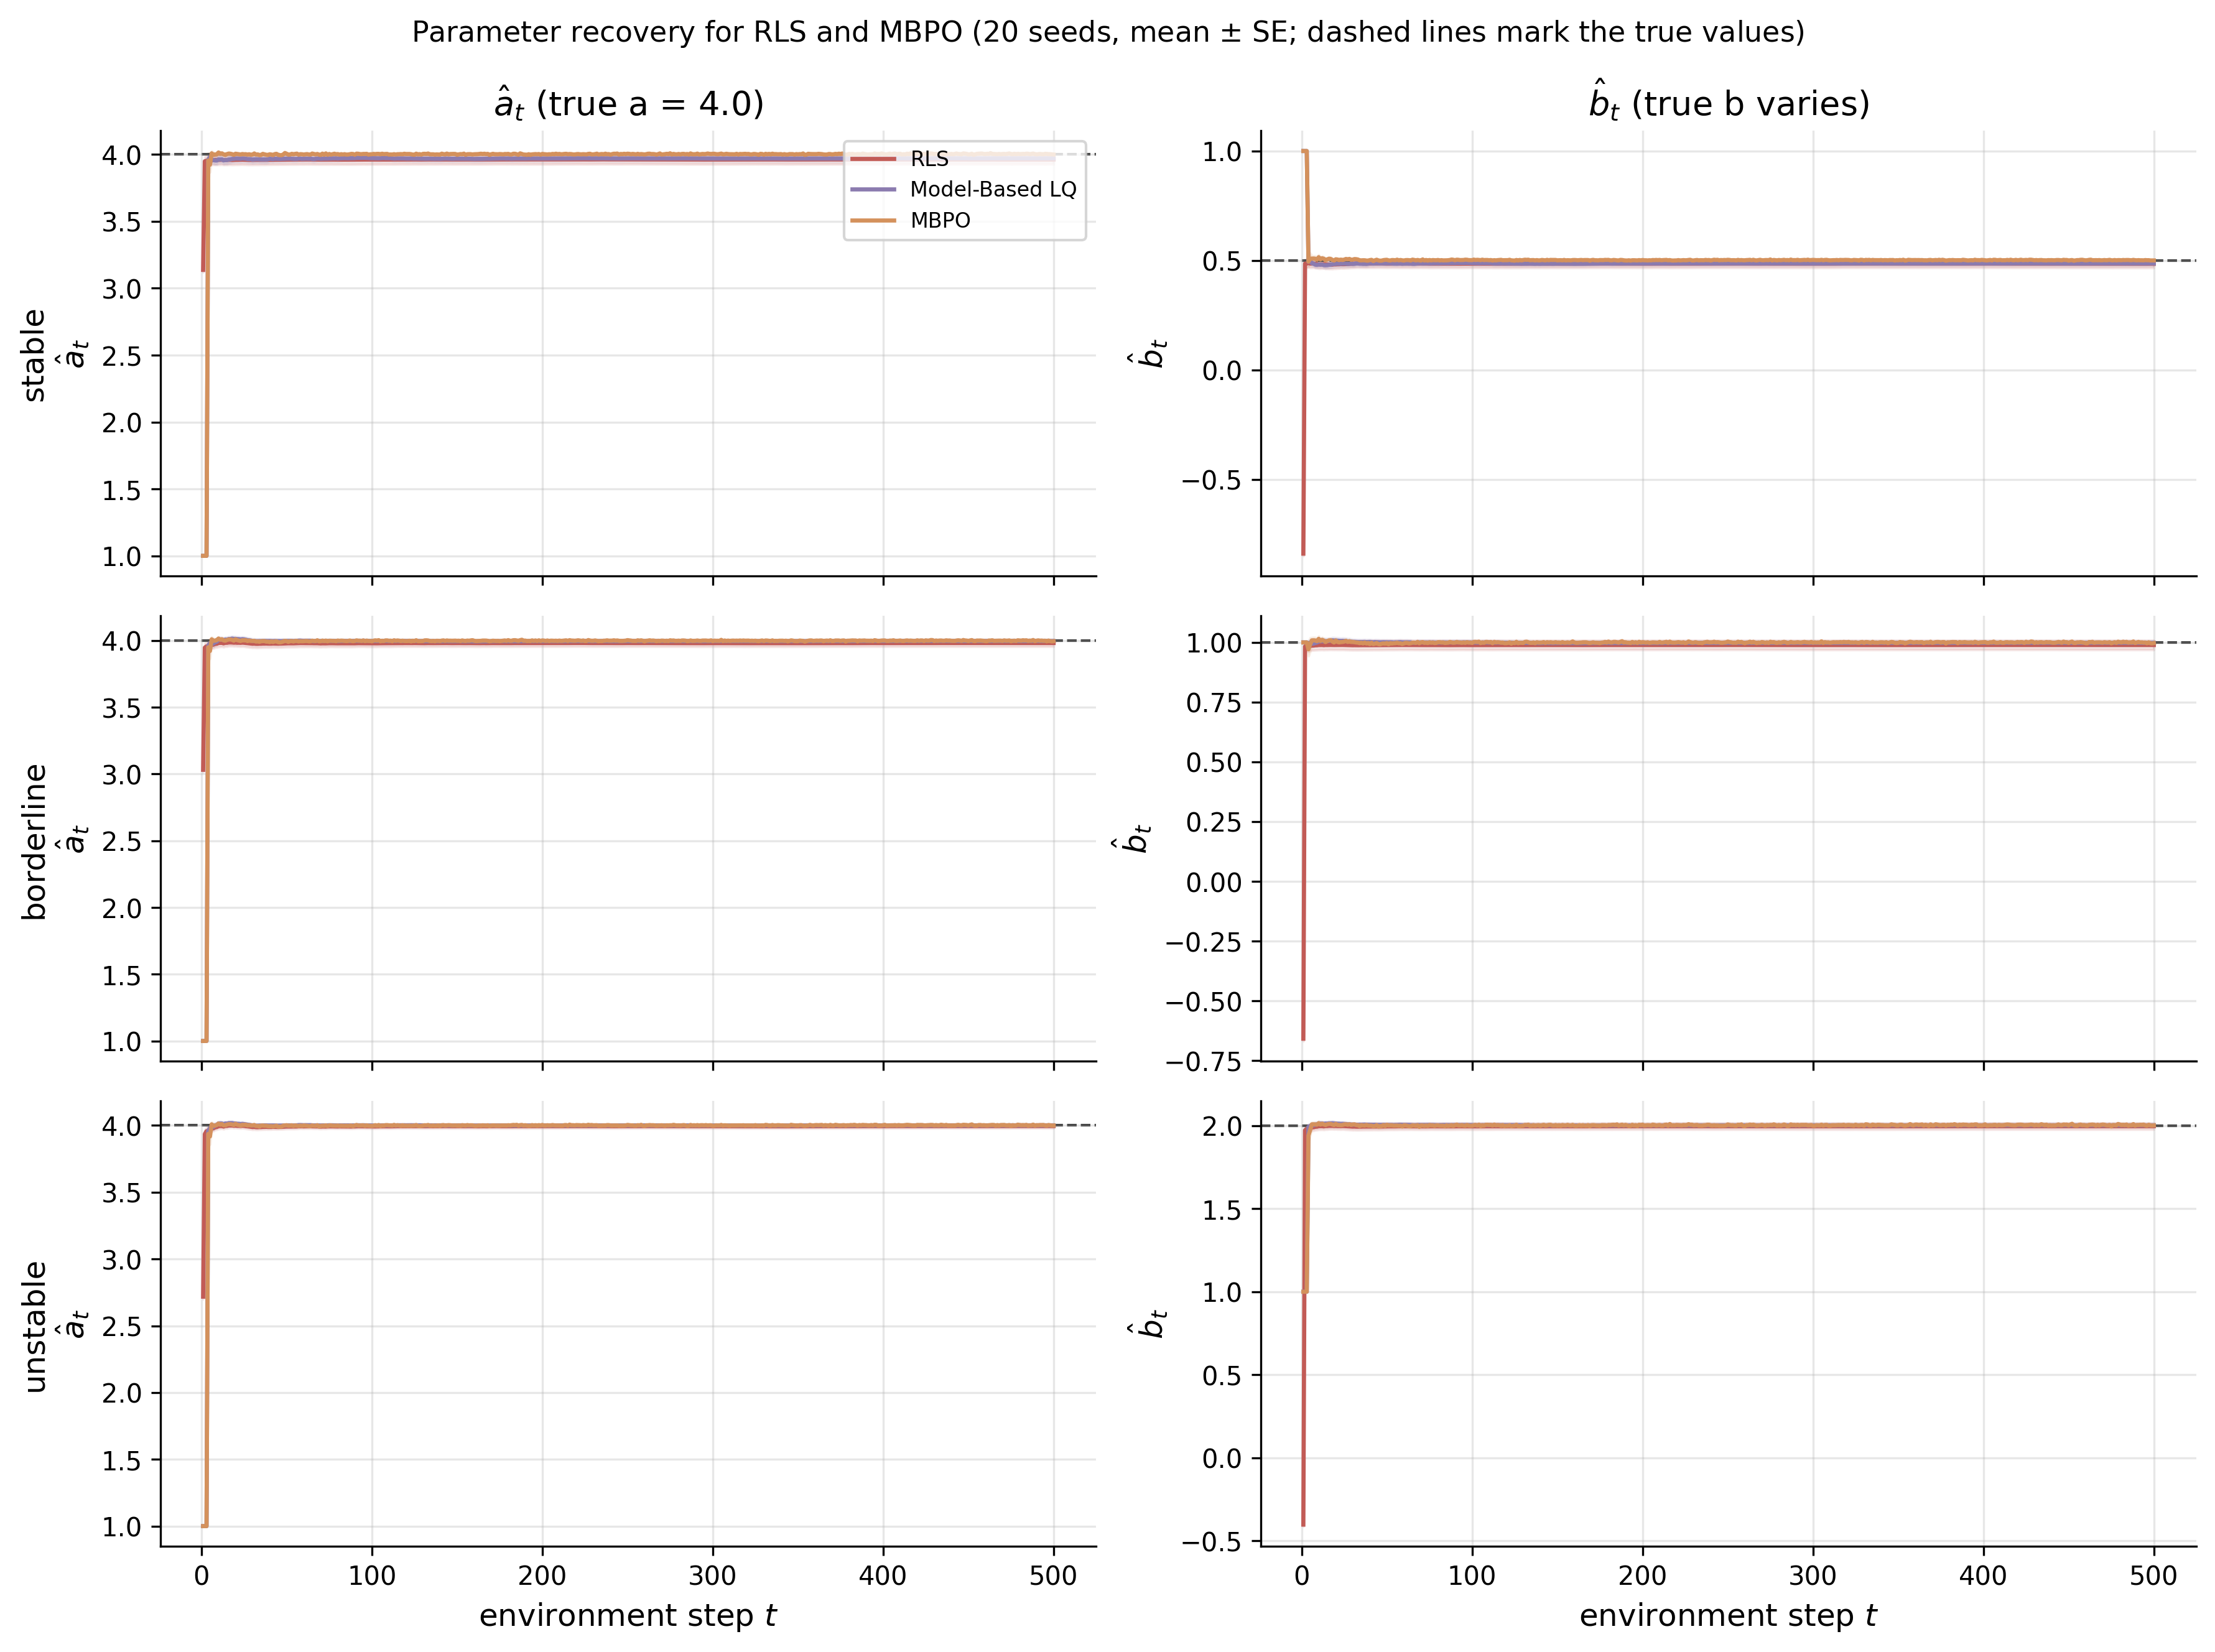
\includegraphics[width=\textwidth]{../ch12_world_models/sims/cobweb_paradigms_param_recovery.png}
  \caption{Parameter recovery for recursive least squares, the model-based LQ learner, and the MBPO ensemble mean across stability regimes. Solid lines are means and shaded bands one standard error across twenty seeds; dashed horizontal lines mark the true values of $a$ and $b$. All three methods converge to the truth within a few dozen environment steps.}
  \label{figure:fc_cobweb_recovery}
\end{figure}

\begin{table}[ht]
  \centering
  \caption{Final parameter recovery error $|\hat\theta - \theta|$ at $t = T$, mean $\pm$ standard error across twenty seeds. Cells marked --- indicate parameters the paradigm does not estimate (recursive least squares assumes $c$ and $\phi$ known); both model-based learners estimate all four.}
  \label{table:fc_cobweb_recovery}
  % Final parameter recovery error |hat - true|, mean +/- SE over 20 seeds.
\begin{tabular}{llcccc}
\toprule
Paradigm & Regime & $|\hat a - a|$ & $|\hat b - b|$ & $|\hat c - c|$ & $|\hat\phi - \phi|$ \\
\midrule
RLS & stable & 0.037 $\pm$ 0.035 & 0.015 $\pm$ 0.018 & --- & --- \\
RLS & borderline & 0.019 $\pm$ 0.026 & 0.011 $\pm$ 0.020 & --- & --- \\
RLS & unstable & 0.004 $\pm$ 0.016 & 0.003 $\pm$ 0.019 & --- & --- \\
\midrule
Model-Based LQ & stable & 0.029 $\pm$ 0.019 & 0.013 $\pm$ 0.009 & 0.000 $\pm$ 0.000 & 0.000 $\pm$ 0.000 \\
Model-Based LQ & borderline & 0.004 $\pm$ 0.011 & 0.002 $\pm$ 0.008 & 0.000 $\pm$ 0.000 & 0.000 $\pm$ 0.000 \\
Model-Based LQ & unstable & 0.001 $\pm$ 0.007 & 0.003 $\pm$ 0.008 & 0.000 $\pm$ 0.000 & 0.000 $\pm$ 0.000 \\
\midrule
MBPO & stable & 0.000 $\pm$ 0.005 & 0.000 $\pm$ 0.002 & 0.000 $\pm$ 0.000 & 0.000 $\pm$ 0.000 \\
MBPO & borderline & 0.005 $\pm$ 0.006 & 0.003 $\pm$ 0.004 & 0.000 $\pm$ 0.000 & 0.000 $\pm$ 0.000 \\
MBPO & unstable & 0.000 $\pm$ 0.005 & 0.002 $\pm$ 0.006 & 0.000 $\pm$ 0.000 & 0.000 $\pm$ 0.000 \\
\midrule
\bottomrule
\end{tabular}

\end{table}

\begin{figure}[ht]
  \centering
  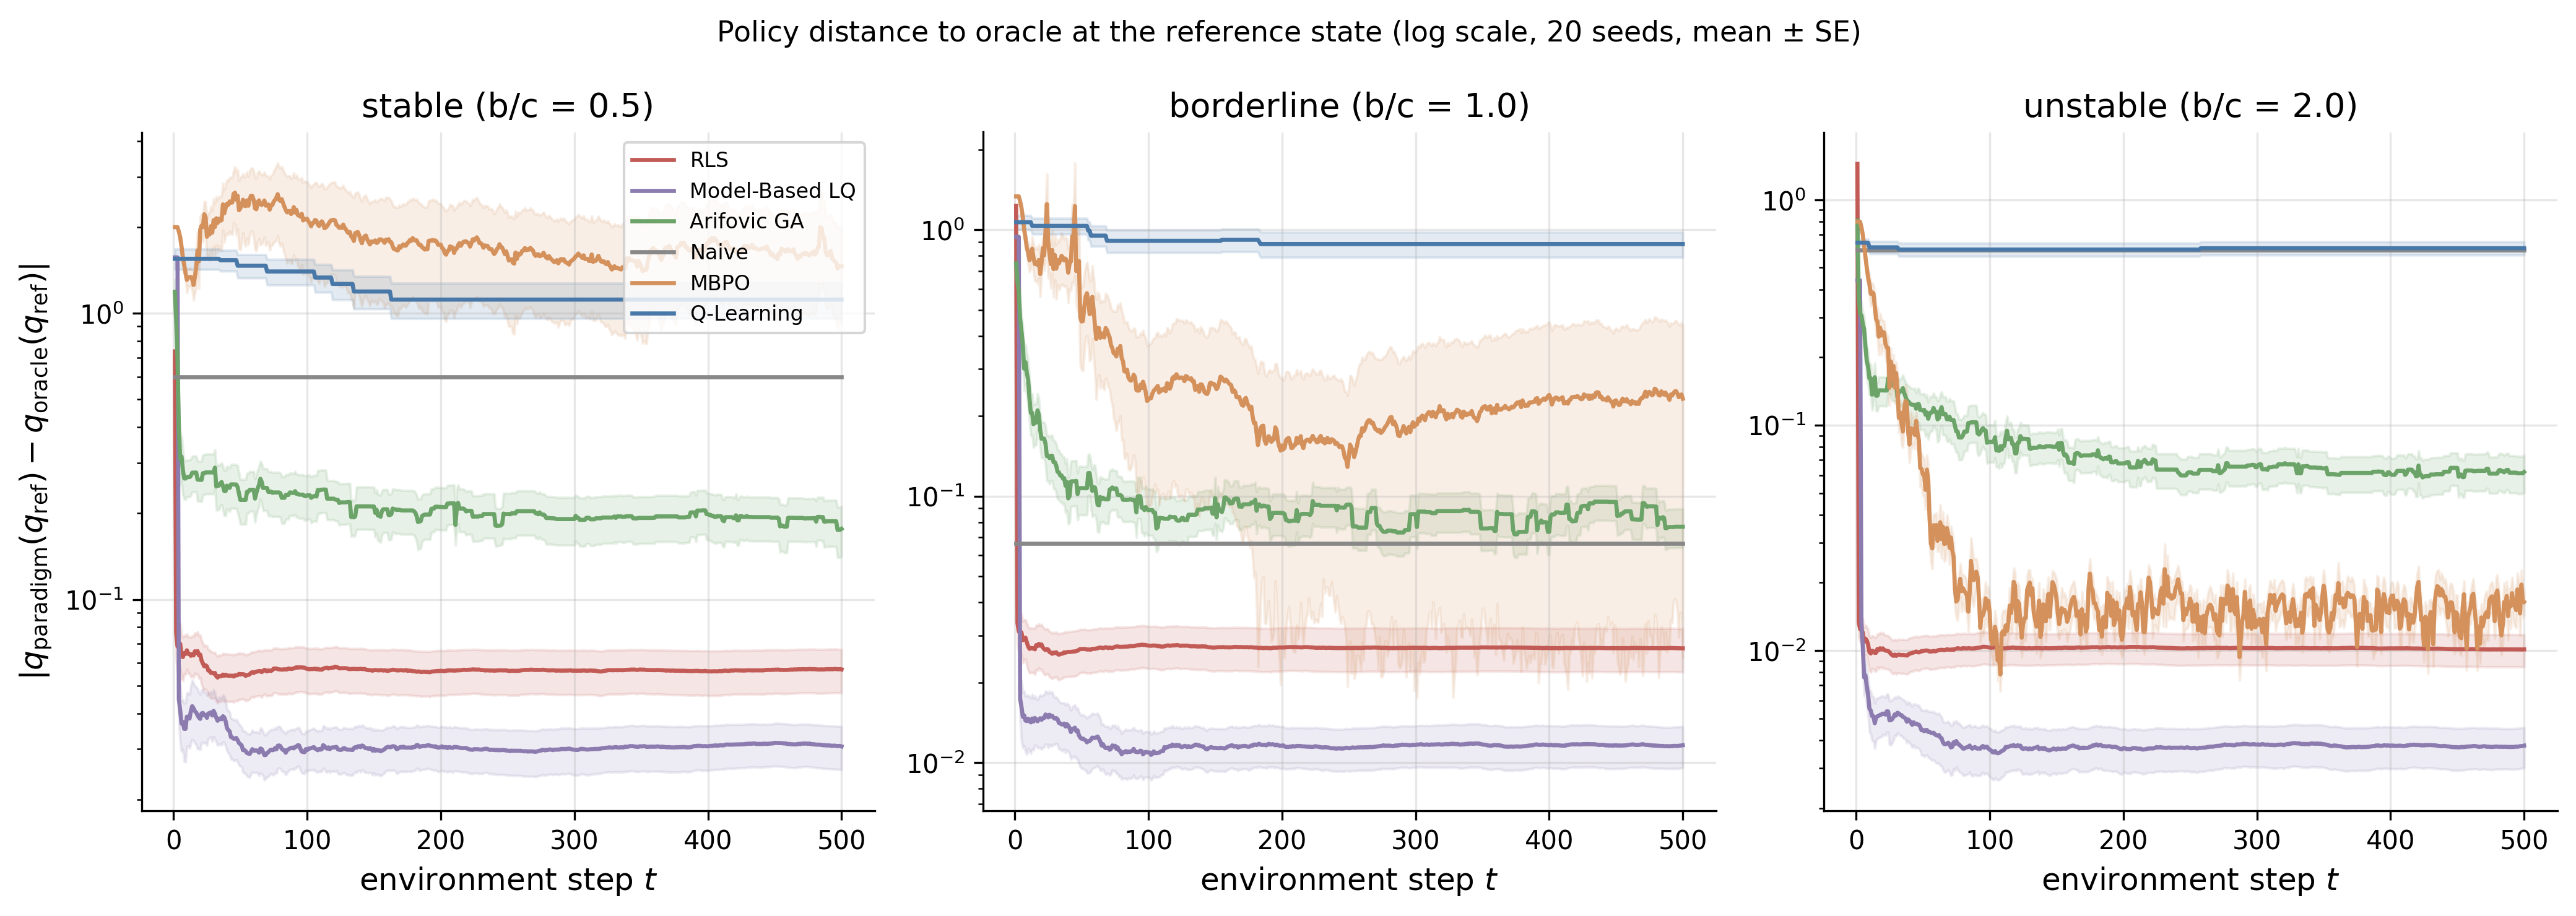
\includegraphics[width=\textwidth]{../ch12_world_models/sims/cobweb_paradigms_policy_distance.png}
  \caption{Policy distance to the oracle at a regime-specific reference state, log scale. The reference state is the static optimum quantity for each regime. Lines are means and bands one standard error across twenty seeds. Oracle is identically zero by construction and is omitted.}
  \label{figure:fc_cobweb_policy_distance}
\end{figure}

\subsubsection{Fishery with logistic growth}
\label{section:fc_dual_sim_fishery}

The fishery panel runs the structured-learner subset of the cobweb's seven paradigms on a logistic-growth fishery, an exogenous environment that isolates the sample-efficiency story from the self-referential pricing of the cobweb. The reward structure is again linear-quadratic, but the transition dynamics are non-linear, so the oracle is a grid-based dynamic-programming solve rather than a closed-form linear-quadratic Riccati.

\paragraph*{Setup.}%
The state is the stock biomass $s_t \in [0, 1.5 K]$ and the action is the harvest $h_t \in [0, \min(s_t, h_{\max})]$. The dynamics are $s_{t+1} = \max(0, s_t + r s_t (1 - s_t / K) - h_t + \varepsilon_t)$ with $\varepsilon_t \sim \mathcal{N}(0, \sigma^2)$, and the reward is $r_t = p h_t - (c/2) h_t^2$. Parameters are $r = 0.4$, $K = 10$, $p = 2.0$, $c = 0.2$, $\sigma = 0.3$, $\gamma = 0.95$, $T = 500$, with twenty independent seeds and $s_0 = K$ (initial stock at carrying capacity). The deterministic maximum-sustainable-yield harvest is $h_{\text{MSY}} = r K / 4 = 1$ at $s^\star = K / 2 = 5$.

\paragraph*{Models.}%
Six paradigms share the budget, a subset of the cobweb panel's seven (the full MBPO with branched rollouts and REINFORCE is omitted here because the fishery's non-linear dynamics make a closed-form policy parameterization unavailable). The oracle solves a grid-based value-iteration discounted dynamic program on $50$ stock $\times$ $25$ action points and applies the greedy policy. The constant-rule baseline plays $h = 0.5$ at every step, a reasonable steady-state guess that lies between zero and the analytic MSY. Recursive least squares estimates $(\hat r, \hat K)$ from a linear-in-parameters regression of $\Delta s_t + h_t$ on $(s_t, -s_t^2)$, plans by re-solving the DP with point estimates every twenty-five observations, and applies the resulting greedy policy with known cost parameters $(p, c)$. The model-based LQ learner estimates $(\hat r, \hat K, \hat p, \hat c)$ jointly by least squares, refits the DP every twenty-five observations, and acts with Gaussian exploration noise that decays over the episode. Tabular Q-learning discretizes $(s, h)$ onto a $30 \times 21$ grid with $\alpha = 0.1$ and $\varepsilon$ decaying from $0.3$ to $0.01$. The genetic algorithm of \citet{Arifovic1994} maintains thirty binary-encoded constant harvest rules and evolves them under fitness-proportional selection and the election operator with known cost parameters.

\paragraph*{Results.}%
Table~\ref{table:fc_fishery_results} reports cumulative regret at $T = 500$ for each paradigm in rank order; Figure~\ref{figure:fc_fishery_curves} shows the regret trajectories. Recursive least squares and the model-based LQ learner sit near the oracle (about thirteen and fifteen regret units respectively), tabular Q-learning recovers a usable policy at roughly two hundred and seventy-five units of regret, the constant rule lands at four hundred and forty-seven, and the genetic algorithm finishes at seven hundred. The fishery's exogenous dynamics give the structured learners a cleaner identification problem than the cobweb because each $(s_t, s_{t+1})$ pair carries direct information about $(r, K)$ that does not get confounded by the agent's own action through expectations, and the consequence is that parameter recovery converges within the first hundred environment steps and the residual regret reflects exploration cost rather than mis-identification. The verdict mirrors the cobweb's inductive-bias frontier with one twist: tabular Q-learning beats both the constant rule and the genetic algorithm on this environment because the discretized state-action grid happens to be coarse enough to be tractable yet fine enough to track the optimal feedback rule's monotone structure, while the genetic algorithm's binary-encoded constant harvest is the wrong functional form for an environment where the optimal action varies smoothly with the stock.

\begin{figure}[ht]
  \centering
  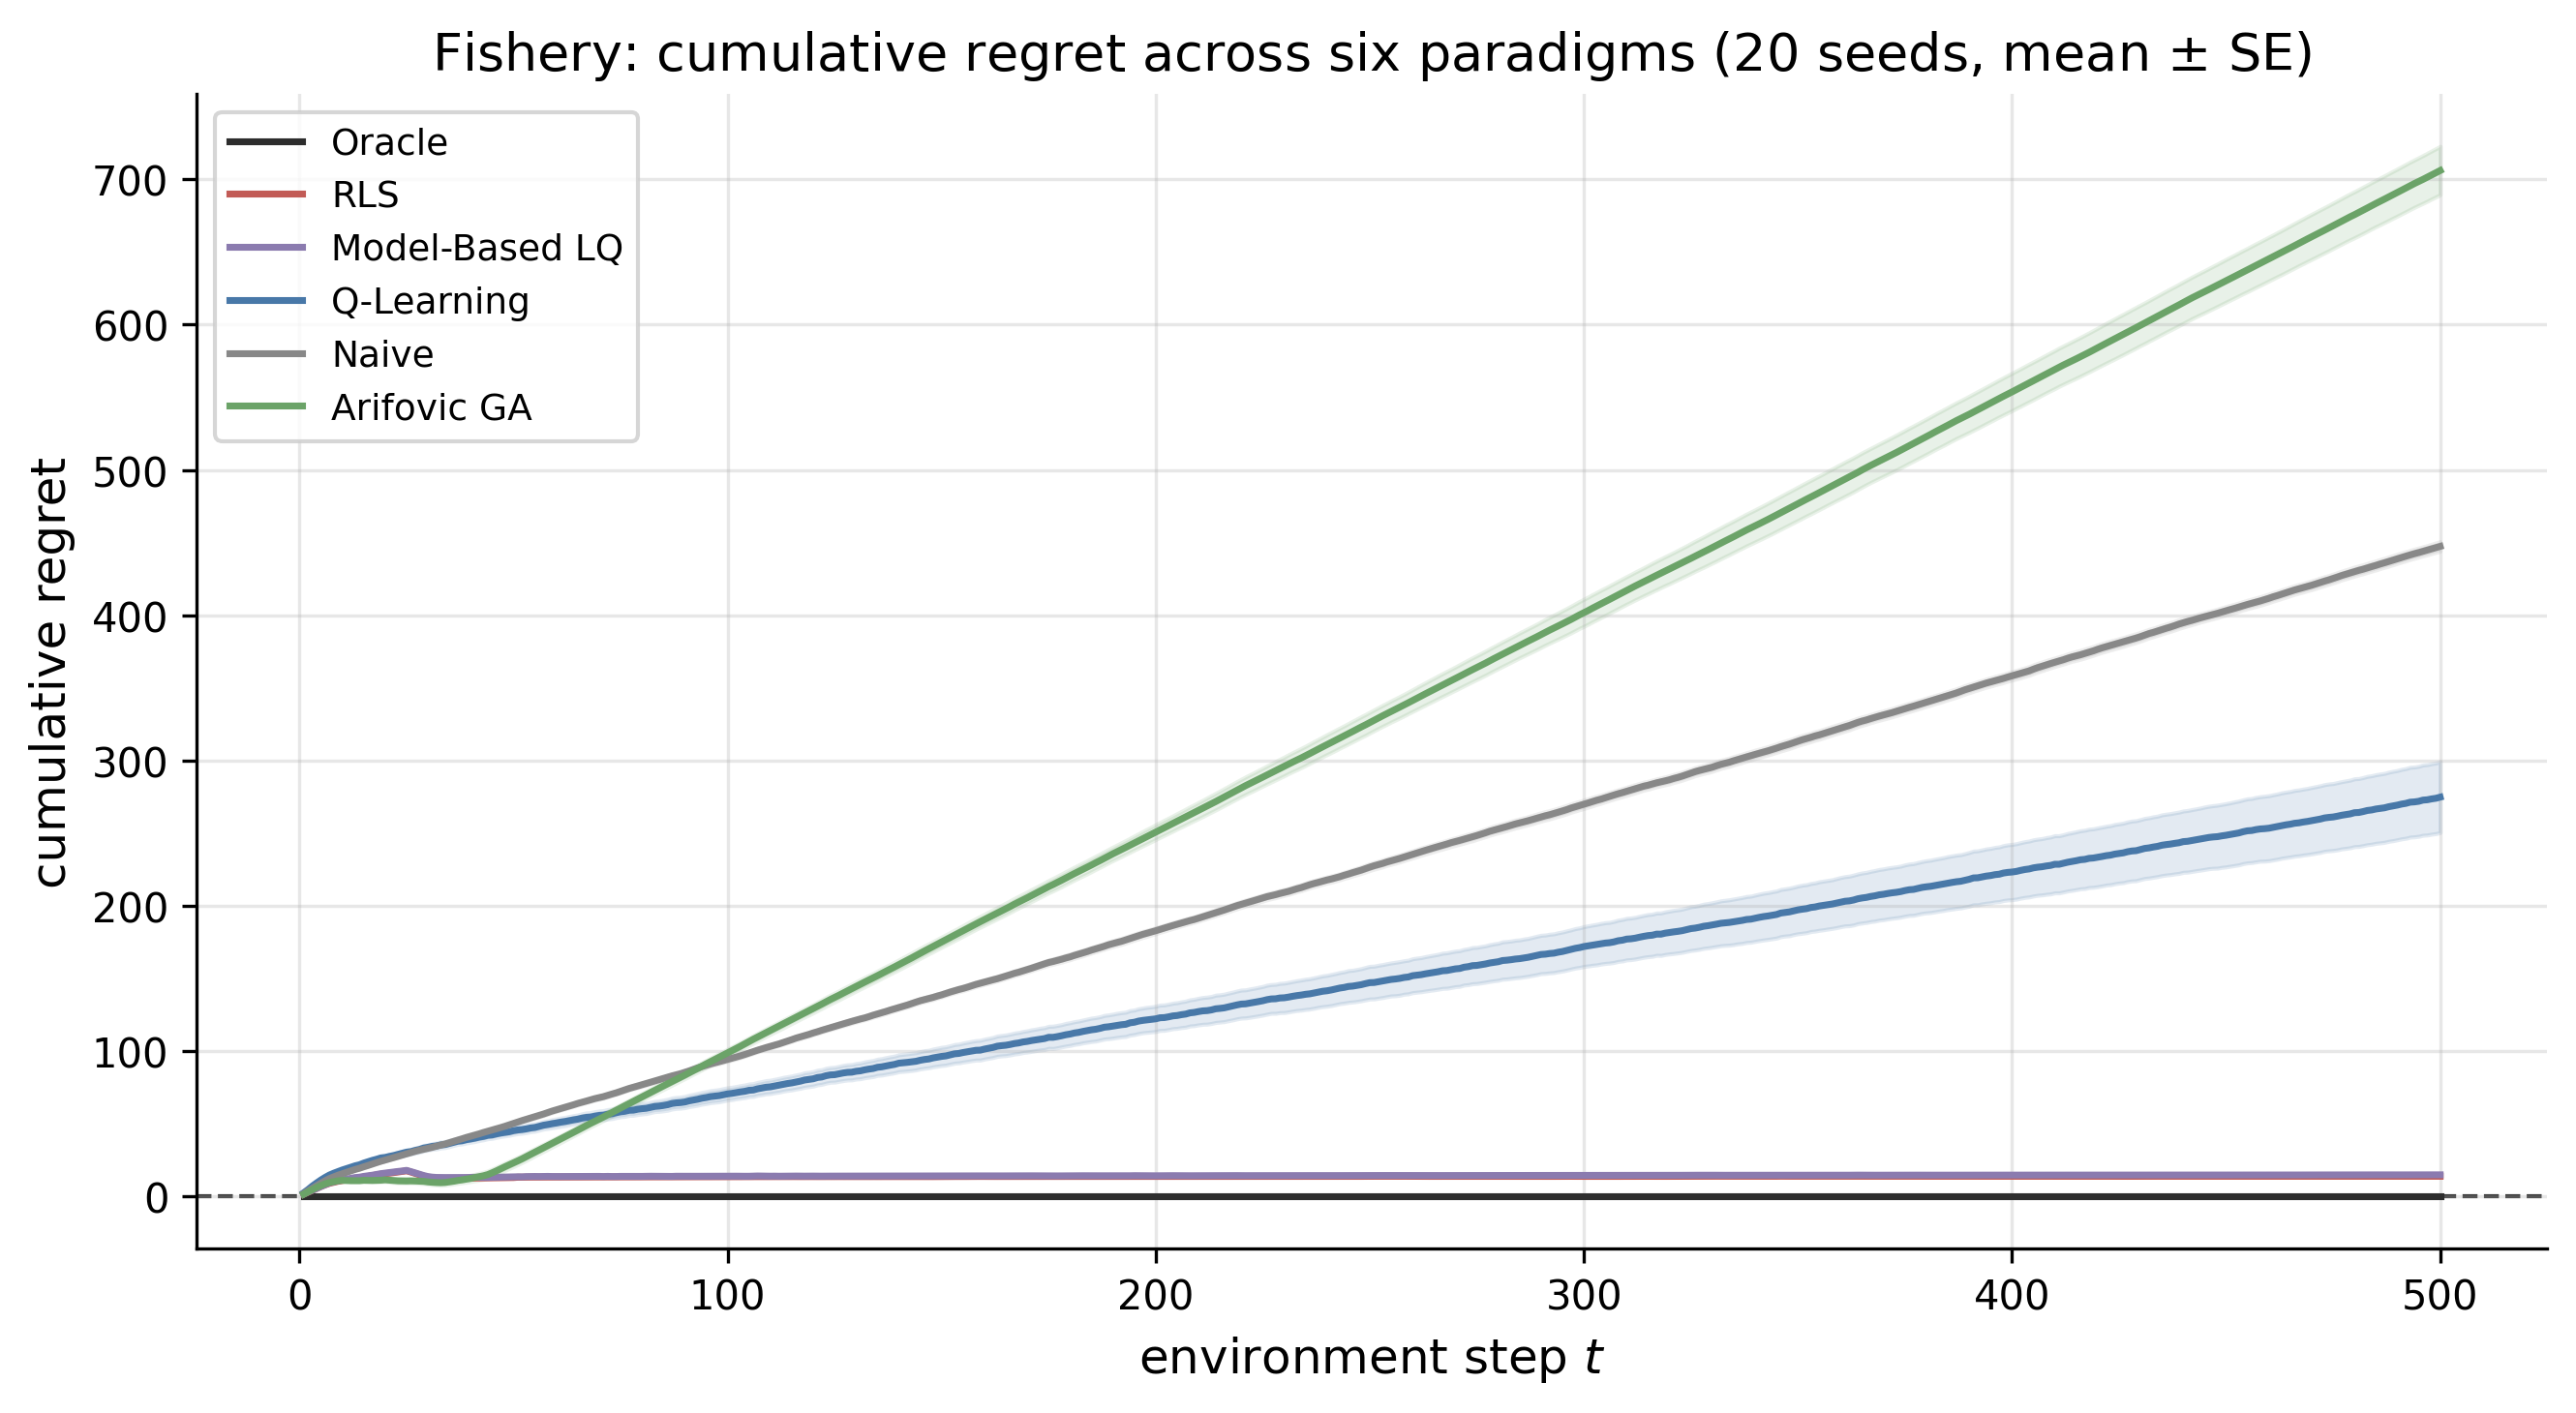
\includegraphics[width=0.95\textwidth]{../ch12_world_models/sims/fishery_paradigms.png}
  \caption{Cumulative regret on the logistic-growth fishery for six paradigms (twenty seeds, mean and one-standard-error bands). Paradigms are presented in rank order by final regret.}
  \label{figure:fc_fishery_curves}
\end{figure}

\begin{table}[ht]
  \centering
  \caption{Final cumulative regret at $T = 500$ on the fishery, mean $\pm$ standard error across twenty seeds. Lower is better; oracle is the zero reference. Paradigms are presented in rank order.}
  \label{table:fc_fishery_results}
  % Cumulative regret at T=500, mean ± SE over 20 seeds.
\begin{tabular}{lr}
\toprule
Paradigm & Final regret \\
\midrule
Oracle & 0.00 $\pm$ 0.00 \\
RLS & 13.67 $\pm$ 0.43 \\
Model-Based DP & 14.69 $\pm$ 0.73 \\
Q-Learning & 274.71 $\pm$ 24.36 \\
Naive & 447.35 $\pm$ 3.24 \\
Arifovic GA & 706.13 $\pm$ 16.65 \\
Myopic & 753.11 $\pm$ 1.75 \\
\bottomrule
\end{tabular}

\end{table}
